%
%

%%-----------------------------------------------------
%%-----------------------------------------------------
\section{¿Cómo sabe mi navegador dónde estoy?}

%%-----------------------------------------------------
\begin{frame}
\frametitle{Pero qué listo es tu móvil}

{\Large
Vete a un sitio donde no haya cobertura GPS

\begin{flushright}
o deshabilita el GPS de tu móvil
\end{flushright}

Lanza la aplicación Google Maps

\begin{flushright}
O busca tu localización en OpenStreetMap

\url{http://www.openstreetmap.org}
\end{flushright}
}

{\huge
\begin{center}
¿Cómo es posible?
\end{center}
}
\end{frame}

%%-----------------------------------------------------
\begin{frame}
\frametitle{Servicios de localización}

{\Large
Bases de datos con coordenadas de puntos de medida de:

\begin{itemize}
\item potencia recibida de puntos de acceso WiFi (MAC, SSID)
\item potencia recibida de estaciones base de redes móviles (CellID)
\end{itemize}

También pueden incluir geolocalización de direcciones IP

\begin{flushright}
\url{http://en.wikipedia.org/wiki/Wi-Fi_positioning_system}
\end{flushright}
}

\end{frame}


%%-----------------------------------------------------
\begin{frame}
\frametitle{Uso de servicios de localización}

{\Large
Ejemplo: Google Play Location Services \\
}
\begin{flushright}
\url{https://developer.android.com/google/play-services/location.html}
\end{flushright}

{\Large
Ejemplo: API JavaScript de Firefox \\
}

\begin{flushright}
\url{https://www.mozilla.org/en-US/firefox/geolocation/} \\
\url{https://developer.mozilla.org/en-US/docs/Web/API/Geolocation/Using_geolocation}
\end{flushright}
\end{frame}

%%-----------------------------------------------------
\begin{frame}
\frametitle{Mozilla Location Service y Stumbler}

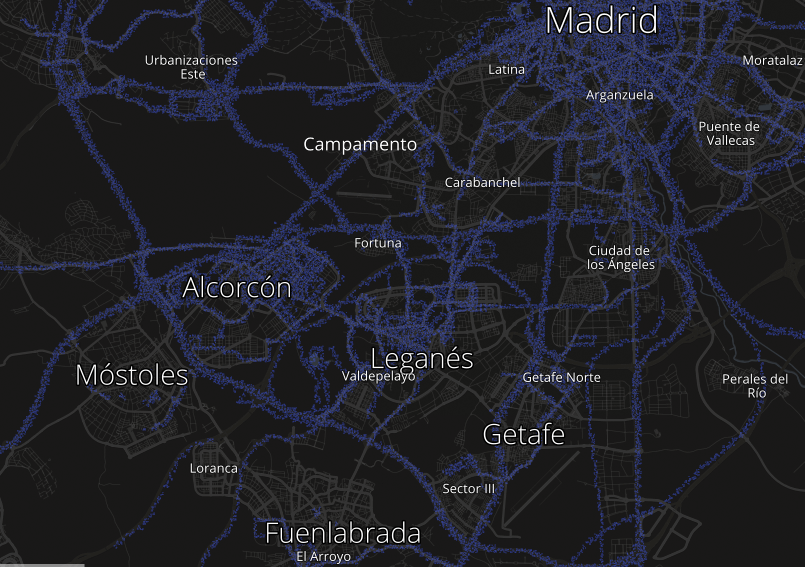
\includegraphics[height=6cm]{figs/mozilla-location-map}

\begin{flushright}
  \url{https://location.services.mozilla.com/map} \\
  \url{https://location.services.mozilla.com/} \\
\end{flushright}
\end{frame}

%%-----------------------------------------------------
\begin{frame}
\frametitle{OpenCellID}

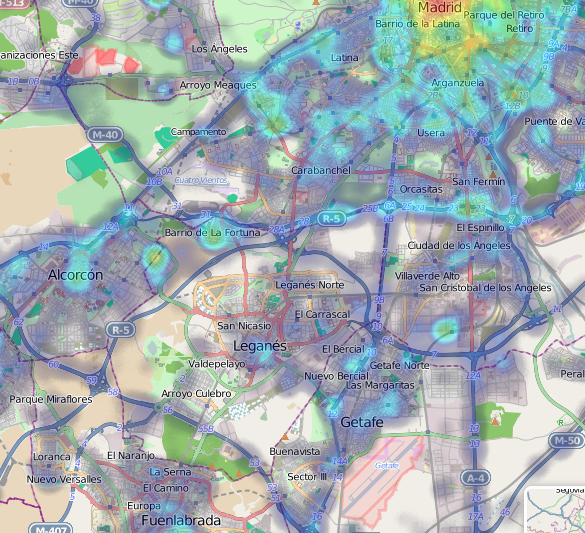
\includegraphics[height=6cm]{figs/opencellid-map}

\begin{flushright}
  \url{http://opencellid.org/} \\
  \url{http://wiki.opencellid.org/wiki/What_is_OpenCellID} \\
  \url{http://wiki.opencellid.org/wiki/Data_sources} \\
\end{flushright}
\end{frame}
